\chapter{Requirements}\label{chap:requirements}

\textcolor{orange}{NOE TEKST}

This chapter presents the requirements provided the \gls{productowner}

This chapter presents a reflection on both the development process and the final product. It examines how the project evolved in relation to the original goals, highlighting what worked well, what could have been improved, and the challenges encountered along the way. The chapter discusses the choice of technologies, project management practices, and team collaboration. It also evaluates the effectiveness and limitations of the final solution, comparing it with existing alternatives and identifying unexpected findings. Broader considerations, such as sustainability and the role of AI in the project, are explored. Finally, the chapter outlines potential directions for future work and improvements to both the product and the project approach.


\section{Project Goals}

This section outlines the overall goal of the project, categorized into product goals, impact goals, and learning goals. Together, these objectives defines the purpose, intended outcomes, and the knowledge expected to be gained through the project process.

\subsection{Product Goals}\label{subsec:req:productgoals}

The primary goal of the project is to develop and test a \textbf{prototype system for fully digital modeling of forestry road load-bearing capacity under varying conditions throughout the year.} The solution will incorporate various geological and meteorological parameters, such as soil type and moisture, weather forecasts, and precipitation data, to generate an accurate classification of forest roads. This classification will be presented through an interactive map-based website. Furthermore, the system will prioritize ease of use, with an intuitive interface designed for transport managers, allowing them to make informed route choices based on real-time data and forecasts. 

\textcolor{orange}{DETTE UNDER ER IKKE NØDVENDIG HER}
The roads will be color-coded using a traffic-light system, where green indicates safe roads, yellow signals caution, and red highlights unsafe roads. The system will provide users with a forecast for road conditions at least a week into the future, enabling better planning and decision-making. 

\subsection{Impact Goals}\label{subsec:req:impactgoals}
% Bærekraft ?
\begin{itemize}
    \item Reduced uncertainty for transport managers when setting the routes using forest roads.
    \item To validate the prototype's feasibility and effectiveness by conducting tests with end-users, such as transport managers, to assess its performance and usability in real-world scenarios.
\end{itemize}

\subsection{Learning Goals}\label{subsec:req:learninggoals}
% Kanskje korte ned litt på dette
% Kanskje oppdatere med noe nytt?? WMS, GIS, osv.
\begin{itemize}
    \item Gaining insight in implementing interactive maps and geospatial data on web pages.
    \item Leveraging RESTful APIs for efficient data integration.
    \item Acquiring hands-on experience collaborating with real-world companies and products.
    \item Gaining experience working in a team environment, improving collaboration and communication skills.
    \item Conducting user tests and implementing feedback. 
    \item Developing a deeper understanding of the software development life cycle while actively practicing agile methodologies, like Scrum and Kanban.
    \item Enhancing application performance by implementing concurrency and optimizing parallel processing.
    \item Expanding proficiency in containerization techniques, particularly through hands-on experience with Docker.
    \item Implementing \Gls{openstack} deployment and configuration using Terraform for efficient infrastructure management.
    % Ikke ta med fra NTNU, heller referer
    \begin{comment}
    \item \textit{\textbf{From NTNU \cite{ntnu_idatg2900}:}}
    \begin{itemize}
        \item Has in-depth knowledge of a selected topic within the subject area.
        \item Has knowledge of research and development work within the topic.
        \item Can identify, formulate and solve a relevant engineering problem.
        \item Can apply knowledge and relevant results from research and development work to solve theoretical, technical and practical problems within the topic of the bachelor thesis and justify their choices.
        \item Can apply engineering methods and work methodically.
        \item Can document and disseminate engineering work.
        \item Can plan and carry out engineering work.
        \item Disseminates professional knowledge to various target groups both in writing and orally in Norwegian and English.
        \item Has insight into scientific honesty and understanding of ethical issues.
        \item Has insight into environmental, health, social and economic consequences of products and solutions within their field and can put these in an ethical perspective and a life cycle perspective.
        \item Integrates previously acquired knowledge and is able to acquire new knowledge in solving a problem.
    \end{itemize}
    \end{comment}
\end{itemize}

\section{Constraints}

\textcolor{orange}{NOE TEKST}

\subsection{Temporal Constraints}

\textcolor{orange}{NOE TEKST}

\begin{itemize}
    \item The set deadline for the final report is 20th of May.
    \item The presentation of the bachelor's thesis is scheduled for 4th or 5th of June.
\end{itemize}

\subsection{Product Constraints}

\textcolor{orange}{NOE TEKST}

\begin{itemize}
    \item The product requires a stable network connection to be used.
    \item The product uses \acrshort{html} 5, which requires newer versions of browsers.
    \item The product needs to be deployed either locally or on a server to run.
\end{itemize}

\begin{comment}
    \subsection{Legal Constraints}
% VET IKKE OM DETTE SKAL VÆRE MED
% ENDRE TIL NÅTID (THE PRODUCT COMPLIES WITH....) ?
\begin{itemize}
    \item The product must comply with the licensing terms and conditions of all third-party services, including map distributors, external APIs, and any code libraries, frameworks, or tools used in its development and deployment.
\end{itemize}
\end{comment}

\section{Project Tasks}
% VET IKKE OM DETTE SKAL VÆRE MED (KANSKJE FJERNE DELER ELLER PEK TIL PROSJEKT PLANEN)
The project aims to develop and test a prototype system for fully digital modeling of forest road load-bearing capacity under varying conditions throughout the year. The development process can be divided into the following areas:

\begin{enumerate}
    \item \textbf{Data Collection and Integration:}
    \begin{itemize}
        \item Decide and gather relevant geological and meteorological data, which may include:
        \begin{itemize}
            \item Superficial deposits, soil moisture, ground water, ground frost.
            \item Weather forecasts.
            \item Historical and real-time road conditions.
        \end{itemize}
        \item Identify and implement suitable data sources and APIs for continuous updates.
    \end{itemize}
    
    \item \textbf{Classification and Forecasting:}
    \begin{itemize}
        \item Develop a rule-based model to classify road conditions based on environmental factors.  
        \item Implement a traffic-light classification system (Green = Safe, Yellow = Caution, Red = Unsafe).  
        \item Extend the model to provide forecasted road conditions at least a week in advance.  
    \end{itemize}
    
    \item \textbf{Web-Based Visual and User Interface:}
    \begin{itemize}
        \item Design and develop an interactive map-based website for intuitive accessibility.
        \item Implement a GIS-based visualization with real-time updates and historical road condition tracking. 
        \item Ensure that the system is optimized for transport managers, with a user-friendly interface that allows efficient decision-making. 
    \end{itemize}
    
    \item \textbf{Testing, Validation and Refinement}:
    \begin{itemize}
        \item Evaluate the accuracy and usability of the system by testing with real-world data.
        \item Conduct user testing with transport managers or forestry stakeholders to assess the effectiveness of the interactive interface and forecasting capabilities.
        \item Incorporate potential user feedback.
    \end{itemize} 
    
    \item \textbf{Documentation and Future Work:}
    \begin{itemize}
        \item Provide detailed documentation of the system architecture, data sources, and model.
        \item Provide a detailed user guide of the product.
        \item Suggest potential improvements, such as machine learning model enhancements, additional data sources, mobile application integration, optimization, or further improvements of the app interface.
    \end{itemize}
\end{enumerate}

\section{Target Audience}

The primary target audience for this application is transport managers in the Norwegian forestry industry. They will use the application to plan routes and determine which forest roads should be used by drivers. Since the user group spans a wide age range, it is essential that the application is intuitive and easy to use, ensuring accessibility for all users regardless of their technical proficiency.

\section{Universal Design}

\textcolor{orange}{NOE TEKST}
\begin{comment}
    Kanskje ikke nødvendig med eget kapittel og kanskje ha det et annet sted? Passer med overgang fra Target Audience ^. SIDEN NOE OM DETTE IKKE BLE NEVNT AV SKOGKURS SÅ BURDE DET KANSKJE STÅ I DISCUSSION I STEDET.
\end{comment}

\section{Use Case}

Use cases provide a clear overview of what a system will and will not do. They enable effective scope management and incremental development, making them well-suited for agile methodologies \cite{jacobson_use_case}. 

This section will present the use case diagram of the system and provide an example of a use case specification.

\subsection{Use Case Diagram}
% DOBBELSJEKK AT SERVEREN IKKE SKAL KOBLES TIL USE CASENE I DIAGRAMMET
The use case diagram shows all interactions the user will have with the website. It also features the application server and its relationship with the external map servers.
\begin{figure}[h]
    \centering
    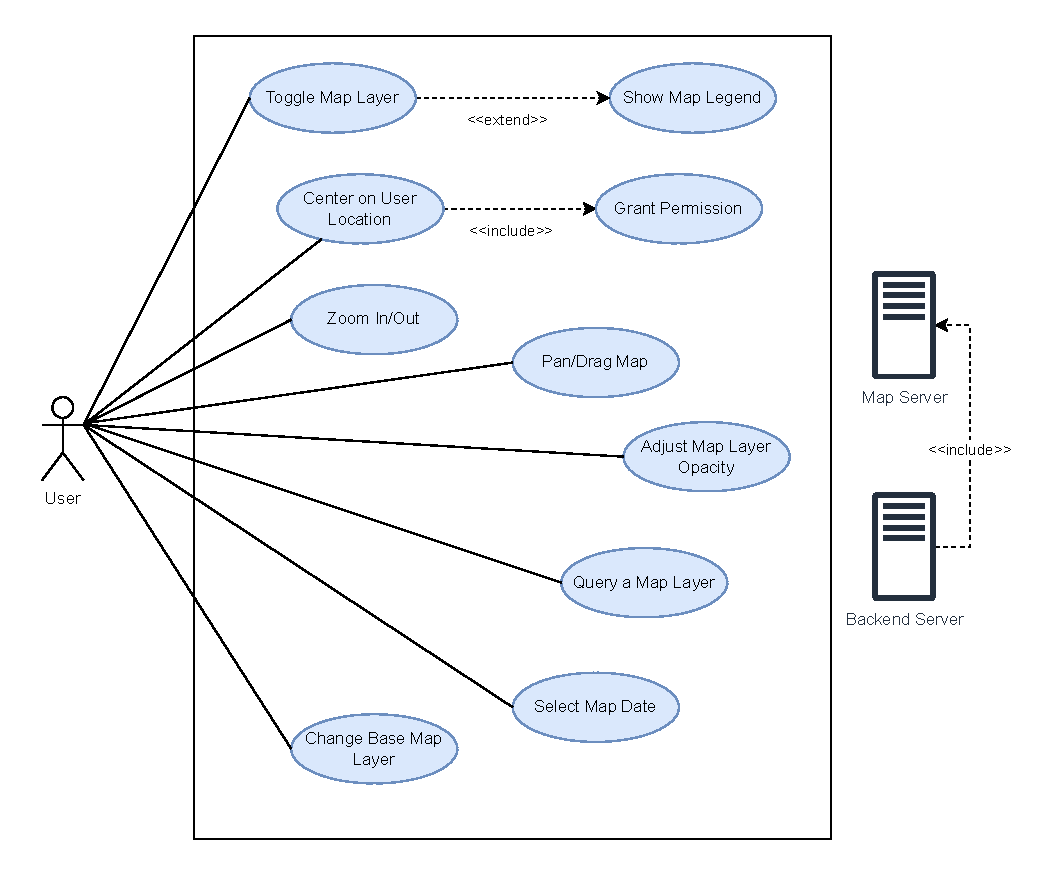
\includegraphics[width=1\linewidth]{figures/use_case_diagram.pdf}
    \caption{Use case diagram of system}
    \label{fig:use_case_diagram}
\end{figure}

\subsection{Actors}

\begin{itemize}
    \item \textbf{User:} The primary user of the website, typically transport managers in the forestry industry, who interact with the system to access relevant map and logistics data.
    \item \textbf{Backend Server:} The central server that the website communicates with to retrieve all necessary map data. It aggregates, processes, and refines data from external services before delivering it to the website.
    \item \textbf{Map Server:} External services that provide map data, either through a \Gls{wms}, \Gls{wfs}, or an \acrshort{api}, which the backend server integrates into the system.
\end{itemize}

\subsection{Use Case Specifications}

It is important to show how users interact with the system to achieve their goals. The use case specifications provide details of each use case and the basic path the user takes to achieve their goals while also capturing possible exceptions. 

A high priority use case for the website is the ability to toggle a map layer, which allows users to control the visibility of different layers. The use case specification for this functionality is shown in \hyperref[tab:use_case_toggle_layer]{Table \ref*{tab:use_case_toggle_layer}}. Additional use case specifications for other features can be found in \hyperref[appendix:use_case_specifications]{Appendix \ref*{appendix:use_case_specifications}}.

\begin{table}[h]
    \centering
    \begin{tabularx}{\textwidth}{|l|X|}
        \hline
        \rowcolor{gray!20}
        \textbf{Use Case Name} & Toggle Map Layer \\
        \hline
        \textbf{Actor(s)} & User \\
        \hline
        \textbf{Description} & The user can toggle specific map layers to control the visibility of different map layers. This functionality allows users to select from various map layers. The selected layer is then displayed, and relevant information is shown in the map legend sidebar. \\
        \hline
        \textbf{Priority} & High \\
        \hline
        \textbf{Pre-Condition(s)} & The user must have a stable internet connection and the website open. The website, server and external map servers must be deployed and running.\\
        \hline
        \textbf{Post-Condition(s)} & The map will be updated with the specific map layer that was toggled. The map legend will also be visible in the legend sidebar. \\
        \hline
        \textbf{Basic Path} &  
        \begin{enumerate}[label=,left=0pt]
            \item 1. User presses the map layer ("kartlag") button to open the map layer sidebar.
            \item 2. User clicks the toggle button for the specific map layer to toggle.
            \item 3. The system updates the map with the selected layer.
        \end{enumerate} \\
        \hline
        \textbf{Exception Path} & 
        \begin{enumerate}[label=,left=0pt]
            \item 0. User does not have a stable internet connection and can not connect to the website.
            \item 2a. Either the backend server or the map server is not responding, and no map data is received.
        \end{enumerate} \\
        \hline
    \end{tabularx}
    \caption[Use Case Specification: Toggle Map Layer]{Use case for toggling a map layer}
    \label{tab:use_case_toggle_layer}
\end{table}
